\documentclass[10pt]{beamer}

\usetheme{default}

\usepackage[utf8]{inputenc}
\usepackage[russian]{babel}
\usepackage[OT1]{fontenc}
\usepackage{amsmath}
\usepackage{amsfonts}
\usepackage{amssymb}
\usepackage{graphicx}
\usepackage{etoolbox}
\usepackage{caption}
\usepackage{subcaption}
\usepackage{pifont}
\usepackage{xcolor}
\usepackage{framed}
\definecolor{shadecolor}{cmyk}{0,0,0,1}
\usepackage{multirow}

\usepackage{listings}

\lstset{
	backgroundcolor=\color{lightgray},
	commentstyle=\color{blue},
	frame=single
	breakatwhitespace, 
	language=python, 
	columns=fullflexible, 
	keepspaces, 
	breaklines, 
	tabsize=3, 
	showstringspaces=false, 
	extendedchars=true,
	numbers=left
}

\makeatletter

\setbeamercolor{title}{fg=white}
\setbeamercolor{frametitle}{fg=black}
\setbeamerfont*{title}{family=\sffamily,size=\LARGE}

\setbeamerfont{page number in head/foot}{size=\scriptsize}
\setbeamertemplate{footline}[frame number]
\let\otp\titlepage
\renewcommand{\titlepage}{\otp\addtocounter{framenumber}{-1}}

\setbeamertemplate{background canvas}{%
	\ifnumequal{\c@framenumber}{0}{%
      
\includegraphics[width=\paperwidth,height=\paperheight]{images/cover.png}
   }{%
      \ifnumequal{\c@framenumber}{\inserttotalframenumber}{
         
\includegraphics[width=\paperwidth,height=\paperheight]{images/back.png}
      }{%
         % Other frames
      }%
   }%
}

\makeatother

\beamertemplatenavigationsymbolsempty

\author{Николай Анохин}
\title{\newline \newline \newline Лекция 6 \\ Линейные модели \\ для классификации и регрессии}

\begin{document}

\begin{frame}[plain]
\titlepage
\end{frame}

\begin{frame}{План занятия}
\tableofcontents
\end{frame}

\begin{frame}{Постановка задачи}

Пусть дан набор объектов $\mathcal{D} = \{(\mathbf{x}_i, y_i)\},
\; \mathbf{x}_i \in \mathcal{X},
\; y_i \in \mathcal{Y},
\; i \in 1, \ldots, N$, полученный из неизвестной закономерности $y = f(\mathbf{x})$. Необходимо выбрать из семейства параметрических функций
\[
H = \{h(\mathbf{x}, \theta): \mathcal{X} \times \Theta \rightarrow \mathcal{Y} \}
\]
такую $h^*(\mathbf{x}) = h(\mathbf{x}, \theta^*)$, которая наиболее точно апроксимирует $f(\mathbf{x})$.

\vspace{1em}
Задачи
\begin{itemize}
\item Регрессия: $\mathcal{Y} = [a, b] \subset \mathbb{R}$
\item Классификация: $|\mathcal{Y}| < C$
\end{itemize}

\end{frame}

% ============================================== %

\section{Линейная регрессия}

% ============================================== %

\begin{frame}{}

\begin{center}
\Large Линейная регрессия
\end{center}

\end{frame}

\begin{frame}{}

\begin{columns}[C]
    \begin{column}{.55\textwidth}
    	Модель
		\[
			y = h(\mathbf{x}, \theta) + \epsilon,
		\]
		где $\epsilon$ -- гауссовский шум
		\[
			p(\epsilon) = \mathcal{N}(\epsilon | 0, \beta^{-1}),
		\]
		откуда
		\[
		p(y | \mathbf{x}, \theta, \beta) = \mathcal{N}(y | h(\mathbf{x}, \theta), \beta^{-1}).
		\]
		Предсказание
		\[
		E[y | \mathbf{x}] = \int y p(y | \mathbf{x}) d y = h(\mathbf{x}, \theta).
 		\]
    \end{column}
       
    \begin{column}{.45\textwidth}
	\begin{center}
   		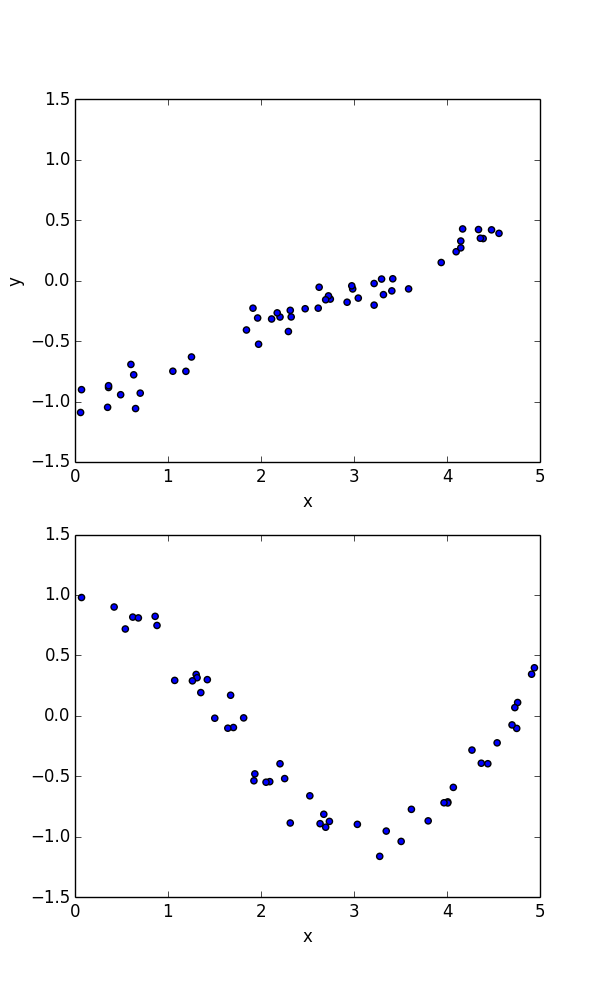
\includegraphics[scale=0.3]{images/empty_reg.png}
    \end{center}
    \end{column}
  \end{columns}

\end{frame}

\begin{frame}{Линейная модель}

\begin{columns}[C]
    \begin{column}{.55\textwidth}
    	простейшая модель
    	\[
    	h(\mathbf{x}, \mathbf{w}) = w_0 + w_1 x_1 + \ldots + w_M x_M = \sum_{j=0}^M w_j x_j
    	\]
    	улучшенная модель
    	\[
    	h(\mathbf{x}, \mathbf{w}) = \sum_{j=0}^M w_j \phi_j(\mathbf{x}) = \mathbf{w}^T \phi(\mathbf{x}),
    	\]
    	$\phi_j(\mathbf{x})$ -- базисные функции, $\phi_0(\mathbf{x}) = 1$ \\ \vspace{1em}
    	примеры
    	\[
    	\varphi_j(x) = x^j, \quad
    	\varphi_j(x) = \exp \left\{-\frac{(x - \mu_j)^2}{2 s^2} \right\}
    	\]
    \end{column}
       
    \begin{column}{.45\textwidth}
	\begin{center}
   		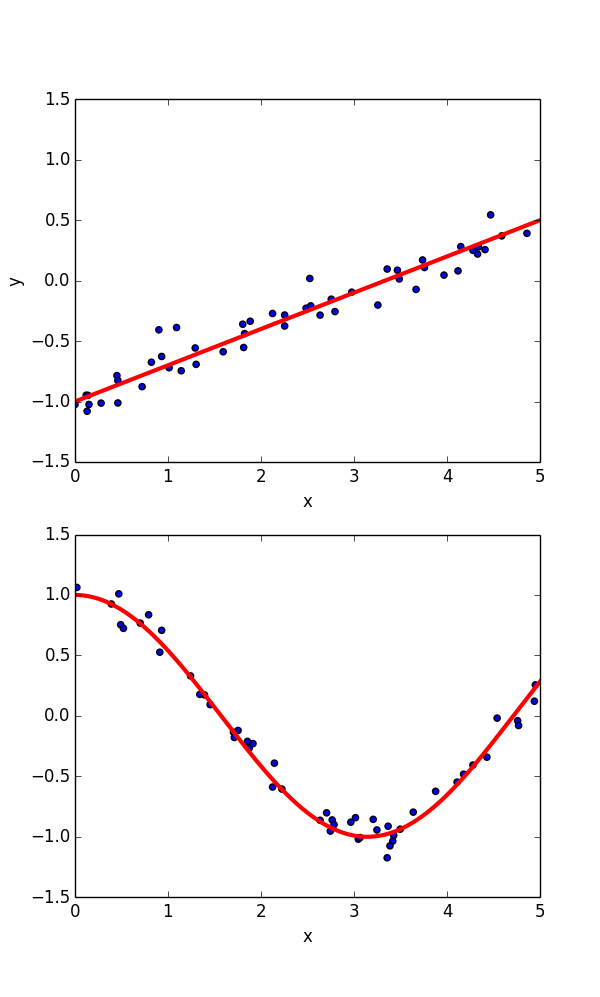
\includegraphics[scale=0.3]{images/full_reg.png}
    \end{center}
    \end{column}
  \end{columns}

\end{frame}

\begin{frame}{ML -- функция правдоподобия}

Дана обучающая выборка $\mathcal{D} = (X, Y)$ из $N$ объектов $(\mathbf{x_n}, y_n)$

\vspace{1em}
Функция правдоподобия
\[
\log p(Y | X, \mathbf{w}, \beta) = \sum_{n=1}^N \log \mathcal{N}(y | \mathbf{w}^T \phi(\mathbf{x_n}), \beta^{-1}) = 
\]
\[
= \frac{N}{2} \log \beta - \frac{N}{2} \log 2 \pi - \frac{\beta}{2} \sum_{n=1}^N \{y_n - \mathbf{w}^T \phi(\mathbf{x}_n)\}^2 \rightarrow \max_{\mathbf{w}, \beta}
\]
Квадратичная функция потерь
\[
E_D(\mathbf{w}) = \frac 1 2 \sum_{n=1}^N \{y_n - \mathbf{w}^T \phi(\mathbf{x}_n)\}^2 \rightarrow \min_{\mathbf{w}}
\]

\end{frame}

\begin{frame}{ML -- решение}

\[
\log p(Y | X, \mathbf{w}, \beta)
= \frac{N}{2} \log \beta - \frac{N}{2} \log 2 \pi - \frac{\beta}{2} \sum_{n=1}^N \{y_n - \mathbf{w}^T \phi(\mathbf{x}_n)\}^2 \rightarrow \max_{\mathbf{w}, \beta}
\]
Градиент
\[
\beta \sum_{n=1}^N \{y_n - \mathbf{w}^T \phi(\mathbf{x}_n)\} \phi(\mathbf{x_n})^T = 0
\]
Решение
 \[
 \mathbf{w}_{ML} = \mathbf{\Phi}^{\dagger} Y = (\mathbf{\Phi}^T \mathbf{\Phi})^{-1} \mathbf{\Phi}^T Y, \quad
 \frac{1}{\beta_{ML}} = \frac{1}{N} \sum_{n=1}^N \{y_n - \mathbf{w}_{ML}^T \phi(\mathbf{x}_n)\}^2, 
 \]
 где
 \[
 \mathbf{\Phi} = \begin{pmatrix}
 \phi_0(\mathbf{x_1}) & \ldots &  \phi_M(\mathbf{x_1}) \\
 \phi_0(\mathbf{x_2}) & \ldots &  \phi_M(\mathbf{x_2}) \\
 \ldots & \ldots & \ldots \\
  \phi_0(\mathbf{x_N}) & \ldots &  \phi_M(\mathbf{x_N}) \\
 \end{pmatrix}
 \]

\end{frame}

\begin{frame}{Регуляризация}

Функция потерь
\[
E(\mathbf{w}, \lambda) = E_D(\mathbf{w}) + \lambda E_W(\mathbf{w}),
\]
где (как и раньше)
\[
E_D(\mathbf{w}) = \frac 1 2 \sum_{n=1}^N \{y_n - \mathbf{w}^T \phi(\mathbf{x}_n)\}^2 \rightarrow \min_{\mathbf{w}},
\]
плюс регуляризация
\[
E_W(\mathbf{w}) = E_q(\mathbf{w}) = \sum_{j=1}^M |\mathbf{w}_j|^q
\]
Зоопарк
\begin{itemize}
\item $q = 1$ -- Lasso
\item $q = 2$ -- Ridge (байесовский вывод: $p(\mathbf{w} | \alpha) = \mathcal{N}(\mathbf{w} | 0, \alpha^{-1} \mathbf{I})$)
\item $E_W(\mathbf{w}) = \rho E_1(\mathbf{w}) + (1 - \rho) E_2(\mathbf{w})$ -- Elastic Net
\end{itemize}

\end{frame}

% ============================================== %

\section{Логистическая регрессия}

% ============================================== %

\begin{frame}{}

\begin{center}
\Large Логистическая регрессия
\end{center}

\end{frame}

% ============================================== %

\section{Обобщенные линейные модели}

% ============================================== %

\begin{frame}{}

\begin{center}
\Large Обобщенные линейные модели
\end{center}

\end{frame}

\begin{frame}{}

\begin{center}
\Large Вопросы
\end{center}

\end{frame}

\end{document}